% =============================================================================
% Module 16: Odd Images, Central Images, and Their Suppression
% =============================================================================
% Part V --- Compound Lenses, Degeneracies, and Cosmography
% Sources: Schneider, Ehlers & Falco (1992) Sect. 5.4.1 (Theorem 1, index
%          theorem, point-mass remark); Petters, Levine & Wambsganss (2001)
%          Sect. 7.4 and Thm 11.4; Congdon & Keeton (2018) Sect. 6.2.2;
%          Burke (1981); Mao, Witt & Koopmans (2001).
% Mathematica: ../Mathematica/16_Odd_Images_Central/odd_images.wl
% Solutions:   ../Solutions/16_Odd_Images_Central/problems_16.wl
% =============================================================================

\chapter{Odd Images, Central Images, and Their Suppression}
\label{ch:odd_images}

\noindent
Chapter~\ref{ch:fermat_time_delays} showed that every image is a
stationary point of the arrival-time surface and stated Burke's
theorem: a smooth, transparent lens produces an odd number of images.
Chapter~\ref{ch:elliptical_models} then walked a source across the
caustics of an elliptical lens and found that the image count changes
by two at each crossing.  Yet the lenses we actually observe are
doubles and quads.  The missing odd image is the \emph{central image},
the maximum of the arrival-time surface, and this chapter is about
where it lives, how faint it is, and what destroys it.

The question is not academic.  Whether a central image exists, and how
bright it is, depends on the innermost tenth or so of the deflector's
Einstein radius: on the size of a core, on the steepness of a cusp, and
on the mass of a central black hole.  The same topology that removes
the central image also removes the radial critical curve, and the
moment at which this happens --- the \emph{annihilation boundary} ---
is the organising idea of Chapter~\ref{ch:central_mass_bias}.  The
degeneracy between a steep inner slope and a central point mass, both
of which suppress the central image, is one reason the inner mass
profile has to be pinned down by other means, the theme of
Chapter~\ref{ch:msd_kinematics}.

By the end of the chapter you should be able to:
\begin{enumerate}[nosep]
    \item sketch the arrival-time surface of a cored lens and locate its
          central maximum;
    \item state exactly which hypothesis of Burke's theorem a point mass
          violates, and what replaces the theorem when it does;
    \item compute the demagnification of the central image and explain
          why observed lenses rarely show one;
    \item see why a central point mass and a steep inner slope both
          suppress it.
\end{enumerate}

\medskip
\noindent
\textbf{Companion Mathematica files:}
\begin{itemize}[nosep]
    \item \mathlink{16_Odd_Images_Central/odd_images.wl}{odd\_images.wl}
          --- symbolic and numerical verification of every result in this
          chapter (Fermat gradient and Hessian, index counting on source
          grids, central-image magnification, point-mass puncture,
          critical black-hole mass); exports the three figures to
          \texttt{Figures/16\_Odd\_Images\_Central/}
    \item \solnlink{16_Odd_Images_Central/problems\_16.wl}{problems\_16.wl}
          --- verified solutions to the Problems
\end{itemize}


% =====================================================================
\section{The Arrival-Time Surface, Revisited}
\label{sec:oi_surface}

We work throughout with the dimensionless Fermat potential of
eq.~\eqref{eq:fermat_potential},
\begin{equation}
    \tau(\vectheta;\vecbeta) = \half|\vectheta-\vecbeta|^2 - \psiL(\vectheta),
    \qquad
    \vecalpha = \nabla\psiL, \qquad \kappab = \half\nabla^2\psiL .
    \label{eq:oi_tau}
\end{equation}
Its gradient is $\nabla\tau = (\vectheta-\vecbeta)-\vecalpha$, so
$\nabla\tau=0$ is the lens equation (eq.~\ref{eq:lens_eq_fermat}), and
its Hessian is the Jacobian matrix, $\partial_a\partial_b\tau = \Amat_{ab}$
(eq.~\ref{eq:hessian_tau}).  Both facts are re-verified for an arbitrary
potential in checks A.1--A.4 of \texttt{odd\_images.wl}.

\begin{bridge}[Back to Chapter~\ref{ch:fermat_time_delays}]
Everything in this chapter is built on three results proved in
Chapter~\ref{ch:fermat_time_delays}: images are stationary points of
$\tau$ (Section~\ref{sec:fermat_principle}); the type of each stationary
point --- minimum, saddle, maximum --- is read off the signs of the two
eigenvalues of $\Amat$ (Table~\ref{tab:morse_types}); and for a smooth
lens $n_{\min}-n_{\rm sad}+n_{\max}=1$ (Theorem~\ref{thm:odd_number}).
We do not re-derive them.  What is new here is (i) a proof of the
counting rule that survives singular lenses, and (ii) the quantitative
fate of the one image the rule forces on us.
\end{bridge}

\subsection{Where can a maximum sit?}

With the shear components $\gamma_1,\gamma_2$ and
$|\gammaL|=(\gamma_1^2+\gamma_2^2)^{1/2}$, the Jacobian
$\Amat=\begin{pmatrix}1-\kappab-\gamma_1&-\gamma_2\\-\gamma_2&1-\kappab+\gamma_1\end{pmatrix}$
has eigenvalues
\begin{equation}
    \lambda_\pm = 1-\kappab \pm |\gammaL| .
    \label{eq:oi_eigen}
\end{equation}
A maximum of $\tau$ needs both eigenvalues negative, i.e.\ the larger
one, $1-\kappab+|\gammaL|$, must be negative:
\begin{equation}
    \boxed{\;\text{maximum of }\tau \;\Longleftrightarrow\; \kappab > 1 + |\gammaL| \;}
    \label{eq:oi_max_condition}
\end{equation}
\annot{checks A.5--A.6}.  A Type~III image can therefore only sit where the
lens is locally \emph{supercritical by more than the shear}.  In a
galaxy this happens only near the centre, which is why the third image
is called the central image.  By the same algebra a minimum needs
$\kappab<1-|\gammaL|$, and a saddle needs $|1-\kappab|<|\gammaL|$
\annot{check A.8}.

\begin{annotation}[Sketching $\tau$ in your head]
Think of $\tau$ as the sum of two surfaces.  The geometric term
$\half|\vectheta-\vecbeta|^2$ is a round bowl centred on the source.
The potential term $-\psiL$ is a hill centred on the lens: $\psiL$ grows
outward (like $\theta$ for an isothermal lens, $\ln\theta$ for a point
mass), so $-\psiL$ is highest at the lens centre.  Far from the lens the
bowl wins and $\tau$ rises like $\half\theta^2$.  Near the centre the
hill can win \emph{if it is sharply peaked}, and its summit is then a
local maximum of $\tau$ --- the central image.  How sharply peaked is
measured by the curvature of $\psiL$, i.e.\ by $\kappab$: that is the
content of eq.~\eqref{eq:oi_max_condition}.  A rounded summit (a core)
gives a genuine maximum; a conical summit (SIS) gives a tip with no
horizontal tangent plane; an infinitely tall spike (point mass) turns
the summit into a puncture.  Between the summit and the minimum there
must be a pass --- the saddle.
\end{annotation}

\subsection{The one-dimensional cut}
\label{sec:oi_cut}

For an axisymmetric lens every image lies on the line through the lens
centre and the source.  Put the source at $\vecbeta=(\ysrc,0)$ with
$\ysrc\ge 0$ and let $\theta$ be a \emph{signed} coordinate along that
line, so that images on the far side of the lens have $\theta<0$.  The
deflection $\alpha(\theta)$ is then an odd function, and the cut through
the arrival-time surface is
\begin{equation}
    \tau(\theta) = \half(\theta-\ysrc)^2 - \psiL(|\theta|), \qquad
    \deriv{\tau}{\theta} = \theta - \ysrc - \alpha(\theta).
    \label{eq:oi_tau_cut}
\end{equation}
The Hessian does not depend on $\ysrc$ (apart from a constant, the source
enters $\tau$ only through the linear term $-\vecbeta\cdot\vectheta$), so
at any point its eigenvalues are those of
Chapter~\ref{ch:axisymmetric_models}, eq.~\eqref{eq:eigenvalues_circular}:
\begin{equation}
    \lambda_r = \deriv{\ysrc}{\theta} = 1-\deriv{\alpha}{\theta}, \qquad
    \lambda_t = 1-\frac{\alpha(\theta)}{\theta},
    \label{eq:oi_lambdas}
\end{equation}
where $\ysrc(\theta)=\theta-\alpha(\theta)$ is the one-dimensional lens
map.  $\lambda_r$ is the curvature of $\tau$ \emph{along} the cut and
$\lambda_t$ its curvature \emph{across} the cut.  Reading off the type
of an image is therefore a two-step exercise: find where
$\ysrc(\theta)$ crosses the source value (the image), and ask whether
$\ysrc(\theta)$ is rising ($\lambda_r>0$) or falling ($\lambda_r<0$)
there and whether the image is outside ($\lambda_t>0$) or inside
($\lambda_t<0$) the tangential critical circle.

\begin{derivation}[Why $\lambda_t$ is the transverse curvature]
For an axisymmetric $\psiL(\theta)$, set
$F(\vectheta)=\half|\vectheta|^2-\psiL(|\vectheta|)$, which differs from
$\tau$ only by the linear term $-\vecbeta\cdot\vectheta$ and a constant,
so it has the same Hessian.  A radial function $F(\theta)$, with
$\hat{\vectheta}=\vectheta/\theta$, has the Hessian
\[
  \partial_a\partial_b F
  = F''(\theta)\,\hat\theta_a\hat\theta_b
  + \frac{F'(\theta)}{\theta}\,\big(\delta_{ab}-\hat\theta_a\hat\theta_b\big).
\]
With $F'=\theta-\alpha$ and $F''=1-\alpha'$ the radial eigenvalue is
$1-\alpha'=\lambda_r$ and the tangential one is
$F'/\theta = 1-\alpha/\theta=\lambda_t$.  On the cut, the tangential
direction is perpendicular to the line through source and lens.
\end{derivation}


% =====================================================================
\section{Counting Images with the Index Theorem}
\label{sec:oi_counting}

Chapter~\ref{ch:fermat_time_delays} quoted the Morse relation
$n_{\min}-n_{\rm sad}+n_{\max}=1$.  To see what happens when the lens
is \emph{not} smooth we need the proof, and the cleanest one is the
index argument of \citet[][Sect.~5.4.1]{schneider_ehlers_falco_1992}.
It uses only the vector field $\mathbf X(\vectheta)=\nabla\tau$.
(The Morse-theoretic version, with Euler characteristics and the Morse
inequalities, is developed in \citealt{petters_singularity_2001},
Sect.~7.4 and Chs.~10--11.)

\paragraph{The index of a stationary point.}
Let $\mathbf X$ be a continuous planar vector field and $c$ a closed
curve on which $\mathbf X\neq 0$.  As we traverse $c$ once
counter-clockwise, the direction angle of $\mathbf X$ turns by $2\pi$
times an integer, the \emph{winding number} of $\mathbf X$ around $c$.
It cannot change while $c$ is deformed without crossing a zero of
$\mathbf X$; the winding number around a small curve enclosing one
isolated zero is the \emph{index} of that zero, and the winding number
around any curve is the sum of the indices of the zeros it encloses.

For $\mathbf X=\nabla\tau$ near an image, $\mathbf X\approx\Amat\,\delta\vectheta$.
In the eigenbasis of $\Amat$ this is $(\lambda_1\,\delta\theta_1,\lambda_2\,\delta\theta_2)$, and
\begin{equation}
    \text{index}(\text{image}) = \operatorname{sgn}(\lambda_1\lambda_2)
    = \operatorname{sgn}\det\Amat = \operatorname{sgn}\mu
    = \begin{cases} +1 & \text{minimum or maximum,}\\ -1 & \text{saddle.}\end{cases}
    \label{eq:oi_index}
\end{equation}

\begin{derivation}[Index of a minimum, a maximum, a saddle]
Take a small circle $\delta\vectheta=\epsilon(\cos\vartheta,\sin\vartheta)$.
Then $\mathbf X=\epsilon(\lambda_1\cos\vartheta,\lambda_2\sin\vartheta)$.
\begin{itemize}
    \item Minimum ($\lambda_1,\lambda_2>0$): $\mathbf X$ points outward
          and its angle increases with $\vartheta$; one loop of
          $\vartheta$ is one loop of $\mathbf X$: index $+1$.
    \item Maximum ($\lambda_1,\lambda_2<0$): $\mathbf X=-\epsilon(|\lambda_1|\cos\vartheta,|\lambda_2|\sin\vartheta)$
          points inward, i.e.\ the outward field rotated by $\pi$; a
          constant rotation does not change the winding: index $+1$.
    \item Saddle ($\lambda_1>0>\lambda_2$): $\mathbf X\propto(|\lambda_1|\cos\vartheta,-|\lambda_2|\sin\vartheta)$,
          whose angle \emph{decreases} as $\vartheta$ increases: index $-1$.
\end{itemize}
A maximum is not the ``opposite'' of a minimum as far as the index is
concerned: both have $\det\Amat>0$.  The index sees only the sign of the
determinant, which is the image parity.
\end{derivation}

\paragraph{The winding at infinity.}
On a circle of radius $R\to\infty$,
$\mathbf X=\vectheta-\vecbeta-\vecalpha(\vectheta)$.  If $|\vecalpha|$
is bounded, the term $\vectheta$ dominates and $\mathbf X$ points
radially outward: its winding number is $+1$.  If, in addition,
$\mathbf X$ is continuous everywhere, the only zeros inside the circle
are the images, so
\begin{equation}
    \sum_{\text{images}}\operatorname{sgn}\mu_i = n_+ - n_- = 1,
    \qquad n_+ = n_{\min}+n_{\max},\;\; n_- = n_{\rm sad}.
    \label{eq:oi_index_sum}
\end{equation}
The total number of images is then
\begin{equation}
    N = n_+ + n_- = 1 + 2\,n_- \qquad (\text{odd}).
    \label{eq:oi_burke}
\end{equation}
This is Burke's odd-number theorem \citep{burke_1981}, in the form of
Theorem~1 of \citet[][Sect.~5.4.1]{schneider_ehlers_falco_1992}.  The
same theorem adds two facts we will use: the global minimum of $\tau$
always exists and is an image, so $n_{\min}\ge 1$; and a source far
enough from the lens has a single image.

\begin{keybox}[The counting rule and its hypotheses]
For a lens whose deflection $\vecalpha(\vectheta)$ is (S1) continuous
everywhere and (S2) bounded, and a source (S3) not on a caustic,
\[
  n_+ - n_- = 1, \qquad N = 1 + 2n_- .
\]
The proof is purely topological: images are the zeros of $\nabla\tau$,
each carries index $\operatorname{sgn}\mu=\pm 1$, and the indices must
add up to the winding of $\nabla\tau$ at infinity.  Hypothesis (S1) is
what a ``smooth, bounded $\Sigma$'' buys in
Theorem~\ref{thm:odd_number}.
\end{keybox}

\begin{bridge}[Back to Chapter~\ref{ch:elliptical_models}]
Section~\ref{sec:image_topology} of Chapter~\ref{ch:elliptical_models}
showed that when a source crosses a fold caustic, two images of opposite
parity appear or disappear together.  In the language of
eq.~\eqref{eq:oi_index_sum} this is obvious: a pair with indices $+1$
and $-1$ contributes zero to the sum, so it can be created from nothing
without changing the winding at infinity.  The quad-plus-one
configuration of Exercise~\ref{ex:burke_verification} has
$n_+=3$, $n_-=2$.  A smooth cored elliptical lens with a source inside
both caustics realises exactly this pattern \annot{checks I.1--I.4; see
Exercise~\ref{ex:oi_five_images}}.
\end{bridge}

\subsection{What the hypotheses exclude}
\label{sec:oi_hypotheses}

Every step above is innocent \emph{except} the claim that the images
are the only zeros of $\mathbf X$ inside the large circle.  That claim
needs (S1).  If $\vecalpha$ fails to be continuous at some point,
the field $\mathbf X$ is undefined there, and that point can carry a
winding of its own even though it is not an image.
Table~\ref{tab:oi_centres} lists the three axisymmetric centres we need.

\begin{table}[ht]
\centering
\caption{The centre of three axisymmetric lenses, seen by the index
theorem.  ``Centre index'' is the winding number of $\nabla\tau$ around
a small circle about a \emph{singular} centre (one that is not an
image).  Verified in \texttt{odd\_images.wl}, checks C.5, E.5--E.7, F.1--F.4.}
\label{tab:oi_centres}
\small
\begin{tabular}{lllll}
\toprule
Lens & $\vecalpha$ near $0$ & $\tau$ near $0$ & Centre index & $n_+-n_-$ \\
\midrule
NIS (core $\theta_c$) & $\kappab_0\,\vectheta$, continuous & smooth summit
    & none (not singular) & $1$ \\
SIS & $\thetaE\,\hat{\vectheta}$, jumps & conical tip
    & $1$ if $|\vecbeta|<\thetaE$, else $0$ & $0$ or $1$ \\
point mass & $\thetaBH^2\,\vectheta/\theta^2$, unbounded & spike, $\tau\to+\infty$
    & $1$ always & $0$ \\
\bottomrule
\end{tabular}
\end{table}

\paragraph{The point mass.}
For a point mass $\psiL=\thetaBH^2\ln\theta$, so
$\vecalpha=\thetaBH^2\vectheta/\theta^2$ diverges at the origin and
$\tau\to+\infty$ there: the summit of the potential hill has become an
infinitely tall spike.  The surface density is a Dirac delta: it is
\emph{not bounded}, the deflection is neither continuous nor bounded at
the origin, and (S1)--(S2) fail there (they still hold far away, so the
winding at infinity is still $+1$).  Near the origin
$\mathbf X\approx-\thetaBH^2\hat{\vectheta}/\theta$ points straight
inward, like the field around a maximum, so the puncture carries index
$+1$ \annot{check E.5}.  The index sum therefore reads
\begin{equation}
    n_+ - n_- + g = 1, \qquad
    N = 2n_- + 1 - g ,
    \label{eq:oi_index_pm}
\end{equation}
for a lens containing $g$ point masses.
\citet[][Sect.~5.4.1]{schneider_ehlers_falco_1992} put it in words:
each point mass turns what would have been a local maximum of $\tau$
into a logarithmic spike, so the number of positive-parity images
\emph{plus the number of point masses} exceeds the number of
negative-parity images by one.  The same counting formula, written as
$N=2n_++g-1$, is Theorem~11.4 of \citet{petters_singularity_2001}, who
also show that as the source moves far away there are $g$ saddle
images, each approaching one of the point masses.  For a single point
mass ($g=1$) the image count is \emph{even}.

\begin{annotation}[Which hypothesis does a point mass break?]
Students often say ``the point mass is not transparent''.  It is: light
does not hit it.  What fails is (S1)/(S2) at one point: the deflection
diverges like $1/\theta$, so $\nabla\tau$ has a singularity that is
not a zero.  The singularity is an \emph{extra term} in the index
sum, worth $+1$.  Excise a small disc around the origin and count on
what is left (an annulus): the winding at infinity minus the winding
around the hole gives $n_+-n_-=1-1=0$.  Put the puncture back as a
``phantom maximum'' and the total is odd again.  Burke's conclusion is
not violated, it is \emph{relocated}: the odd image has become the
singularity itself.
\end{annotation}

\paragraph{The SIS.}
For the singular isothermal sphere, $\vecalpha=\thetaE\hat{\vectheta}$
has constant length but its direction jumps at the origin: (S1) fails,
(S2) holds.  The surface $\tau$ has a conical tip, a local maximum with
no tangent plane, so it is not a stationary point and produces no
image.  Its index depends on the source: near the origin
$\mathbf X\approx-\vecbeta-\thetaE\hat{\vectheta}$, which winds once if
$|\vecbeta|<\thetaE$ and not at all if $|\vecbeta|>\thetaE$ \annot{checks F.1--F.2}.  This is the index-theorem reading of the SIS ``cut'': two
images ($n_+-n_-=0$) inside it, one image ($n_+-n_-=1$) outside.
Exercise~\ref{ex:oi_sis_tip} asks you to do the computation.

\paragraph{Cusps that are not singular enough.}
A power-law profile $\kappab\propto\theta^{1-\gp}$ with $1<\gp<2$ has an
\emph{infinite} central convergence, so its surface density is not
bounded.  But $\alpha\propto\theta^{2-\gp}\to0$ continuously at the
origin, so (S1) holds, the index argument goes through, and the lens
produces an odd number of images: it has a central image
(Section~\ref{sec:oi_steep}).  What the counting rule really needs is
continuity of the deflection, not finiteness of the density.


% =====================================================================
\section{The Central Image of a Cored Lens}
\label{sec:oi_central}

The non-singular isothermal sphere (NIS) of
Chapter~\ref{ch:axisymmetric_models}, Section~\ref{sec:nis}, is the
simplest lens with a genuine central image.  Its convergence and
deflection are (eqs.~\ref{eq:nis_kappa} and~\ref{eq:nis_alpha})
\begin{equation}
    \kappab(\theta) = \frac{\thetaE}{2\sqrt{\theta^2+\theta_c^2}}, \qquad
    \alpha(\theta) = \thetaE\,\frac{\sqrt{\theta^2+\theta_c^2}-\theta_c}{\theta},
    \label{eq:oi_nis}
\end{equation}
with central convergence $\kappab_0=\thetaE/(2\theta_c)$
(eq.~\ref{eq:nis_kappa_central}).  The potential, needed to draw $\tau$,
is
\begin{equation}
    \psiL(\theta) = \thetaE\Big[s - \theta_c\ln\!\big(\theta_c + s\big)\Big],
    \qquad s\equiv\sqrt{\theta^2+\theta_c^2},
    \label{eq:oi_psi_nis}
\end{equation}
up to an irrelevant constant \annot{checks B.1--B.3: $\psiL'=\alpha$ and
$\half\nabla^2\psiL=\kappab$}.

\begin{bridge}[Back to Chapter~\ref{ch:axisymmetric_models}]
We reuse the NIS exactly as defined in Section~\ref{sec:nis}: $\thetaE$
is the Einstein radius of the SIS the NIS tends to as $\theta_c\to0$,
and the core is supercritical ($\kappab_0>1$) for $\theta_c<\thetaE/2$.
Chapter~\ref{ch:axisymmetric_models} established that a supercritical
core has a radial critical curve and can make three images.  Here we
supply what that chapter left qualitative: the type and arrival order
of each image, the radial caustic in closed form, and the magnification
of the third image.
\end{bridge}

\subsection{Three images, at most}

Multiplying the NIS lens equation $\ysrc=\theta-\alpha(\theta)$ by
$\theta$ and isolating the square root gives
$\thetaE\,s=\theta^2-\ysrc\,\theta+\thetaE\theta_c$; squaring and
discarding the spurious root $\theta=0$ leaves a cubic,
\begin{equation}
    \theta^3 - 2\ysrc\,\theta^2 + \big(\ysrc^2 + 2\thetaE\theta_c - \thetaE^2\big)\theta
    - 2\ysrc\,\thetaE\theta_c = 0
    \label{eq:oi_nis_cubic}
\end{equation}
\annot{checks B.4--B.6}, so the NIS has at most three images.  The radial
critical curve is where $\lambda_r=0$; by eq.~\eqref{eq:oi_theta2lr}
below (at $\thetaBH=0$) it is the positive root of
$s^2+\theta_c s-\thetaE\theta_c=0$:
\begin{equation}
    s_r = \frac{-\theta_c+\sqrt{\theta_c^2+4\thetaE\theta_c}}{2}, \qquad
    \theta_r = \sqrt{s_r^2-\theta_c^2}, \qquad
    \ysrc_r = \big|\theta_r - \alpha(\theta_r)\big| .
    \label{eq:oi_nis_radial}
\end{equation}
For $\theta_c=0.2\,\thetaE$ this gives $\theta_r=0.297\,\thetaE$ and a
radial caustic of radius $\ysrc_r=0.235\,\thetaE$; for
$\theta_c=0.1\,\thetaE$, $\theta_r=0.251\,\thetaE$ and
$\ysrc_r=0.427\,\thetaE$ \annot{checks C.1, C.9, FIG3}.

\paragraph{The census.}
On a grid of 149 source positions $0.01\le\ysrc/\thetaE\le1.5$, the
script finds every root of eq.~\eqref{eq:oi_nis_cubic} and classifies
it with eq.~\eqref{eq:oi_lambdas} \annot{checks C.2--C.8, $\theta_c=0.2\,\thetaE$}:
\begin{itemize}[nosep]
    \item $\ysrc>\ysrc_r$: one image, a minimum;
    \item $\ysrc<\ysrc_r$: three images --- the minimum; a saddle on the far
          side \emph{outside} the radial critical circle
          ($\theta<-\theta_r$); and a maximum on the far side
          \emph{inside} it ($-\theta_r<\theta<0$);
    \item in every case $n_+-n_-=1$;
    \item at $\ysrc=0.1\,\thetaE$ the arrival order is
          $\tau_{\min}<\tau_{\rm sad}<\tau_{\max}$: the central image
          arrives last, as Table~\ref{tab:morse_types} leads us to
          expect for a Type~III image;
    \item as $\ysrc\to\ysrc_r$ from below, the saddle and the maximum
          merge on the radial critical circle and disappear together.
\end{itemize}
The left column of Figure~\ref{fig:oi_arrival} shows the contours of
$\tau$.  The contour through the saddle is a figure eight: one lobe
encloses the central maximum, the other the minimum.

\begin{figure}[ht]
    \centering
    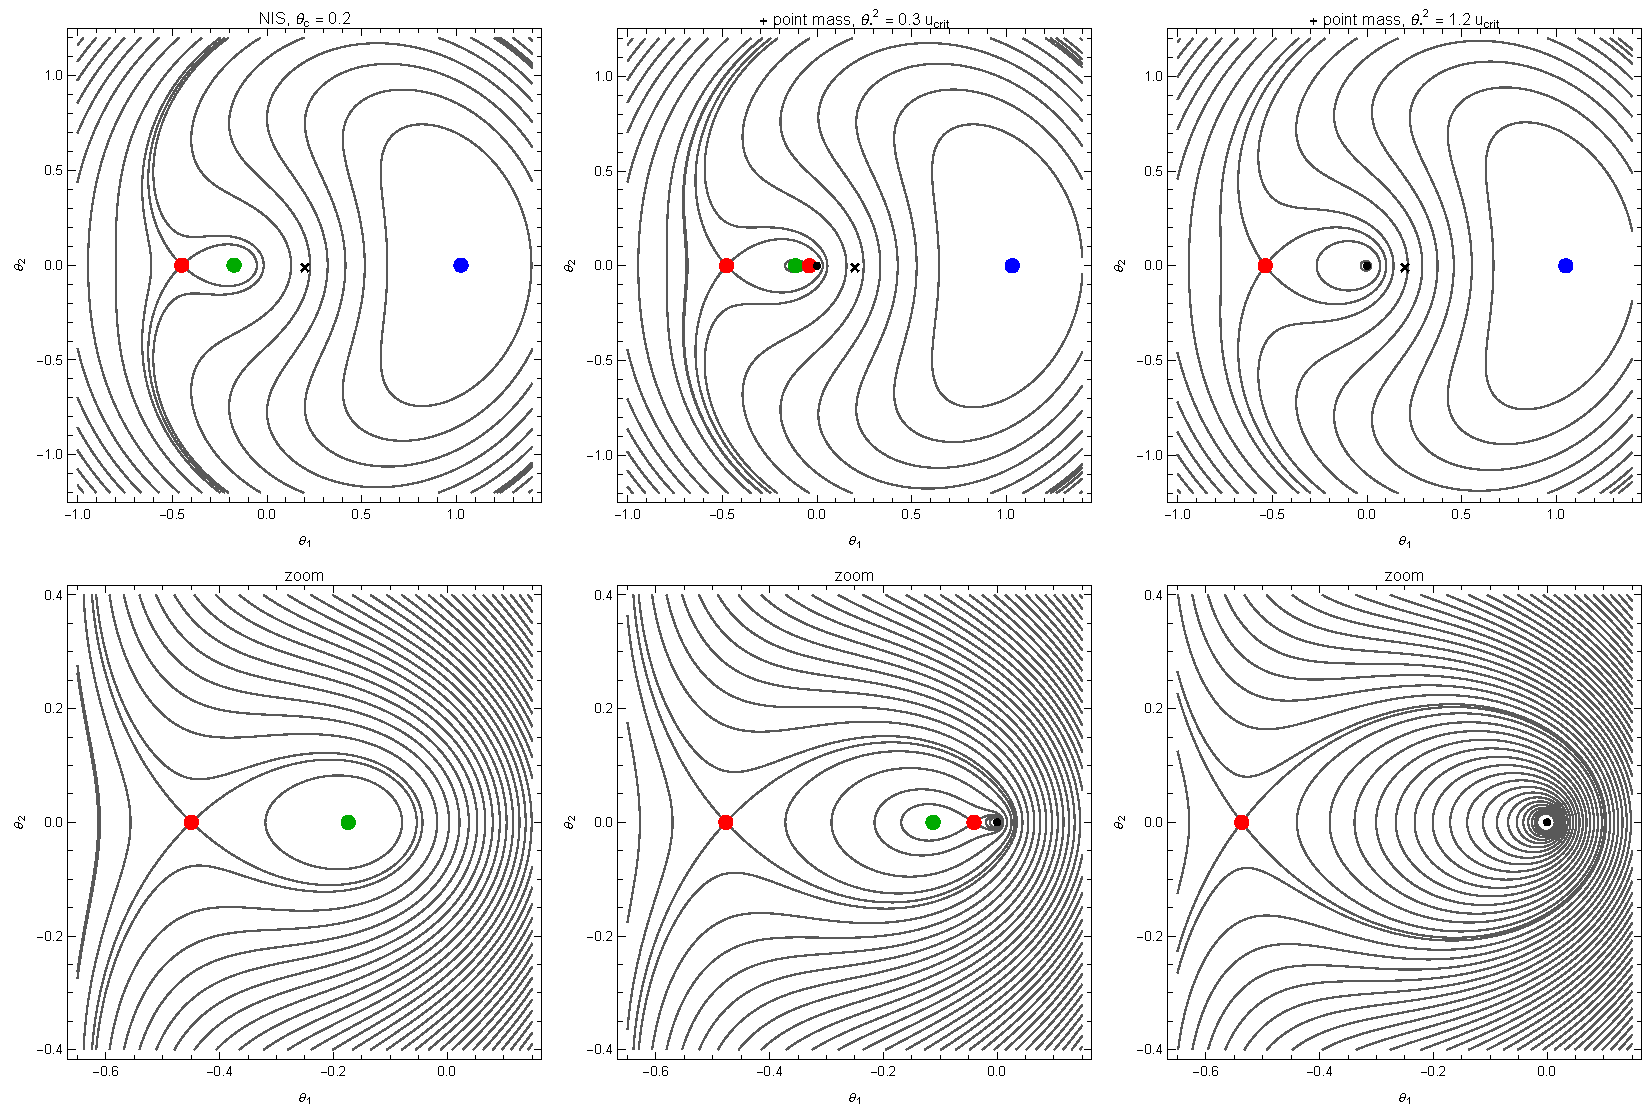
\includegraphics[width=\textwidth]{../Figures/16_Odd_Images_Central/arrival_time_nis_bh.pdf}
    \caption{Contours of the arrival-time surface $\tau(\theta_1,\theta_2)$
    for an NIS with $\theta_c=0.2\,\thetaE$ and a source at
    $\vecbeta=(0.2,0)\,\thetaE$ (black cross); top row full view, bottom
    row zoom on the centre; axes in units of $\thetaE$.
    \textbf{Left:} NIS alone --- minimum (blue), saddle (red), central
    maximum (green).
    \textbf{Centre:} NIS plus a central point mass with
    $\thetaBH^2=0.3\,\theta_{\bullet,\rm crit}^2$ --- the summit is
    punctured (black dot) and a second saddle appears next to the
    puncture; four images.
    \textbf{Right:} $\thetaBH^2=1.2\,\theta_{\bullet,\rm crit}^2$ ---
    the maximum and the inner saddle are gone; two images.  Generated
    by \texttt{odd\_images.wl}.}
    \label{fig:oi_arrival}
\end{figure}

\subsection{How faint is the central image?}

Put the source on the axis, $\ysrc=0$.  The central image is then at
$\theta=0$, where $\alpha(\theta)\simeq\kappab_0\theta$, so both
eigenvalues equal $1-\kappab_0$ (the shear vanishes at the centre of an
axisymmetric lens):
\begin{equation}
    \boxed{\;
    \mu_c = \frac{1}{(1-\kappab_0)^2}
          = \frac{4\theta_c^2}{(\thetaE-2\theta_c)^2}
          = \frac{4\theta_c^2}{\thetaE^2}\left[1+\frac{4\theta_c}{\thetaE}+\mathcal{O}\!\left(\frac{\theta_c^2}{\thetaE^2}\right)\right]
    \;}
    \label{eq:oi_muc}
\end{equation}
\annot{checks D.1--D.5}.  For a source slightly off axis, linearising
$\ysrc\simeq(1-\kappab_0)\theta$ puts the central image at
$\theta\simeq-\ysrc/(\kappab_0-1)$, on the far side and
$\kappab_0-1$ times closer to the centre than the source, with the same
magnification to leading order \annot{checks D.8--D.9}.  The magnification falls
as the \emph{square} of the core radius: a core one hundred times
smaller than the Einstein radius makes the central image
$\mu_c=1/2401$ times as bright as the unlensed source, $8.5$ magnitudes
fainter; even a generous core, $\theta_c=0.1\,\thetaE$, gives
$\mu_c=1/16$, $3.0$ magnitudes fainter \annot{checks D.6--D.7}.
Figure~\ref{fig:oi_muc} shows eq.~\eqref{eq:oi_muc} against a direct
numerical solution at $\ysrc=0.1\,\thetaE$.

\begin{figure}[ht]
    \centering
    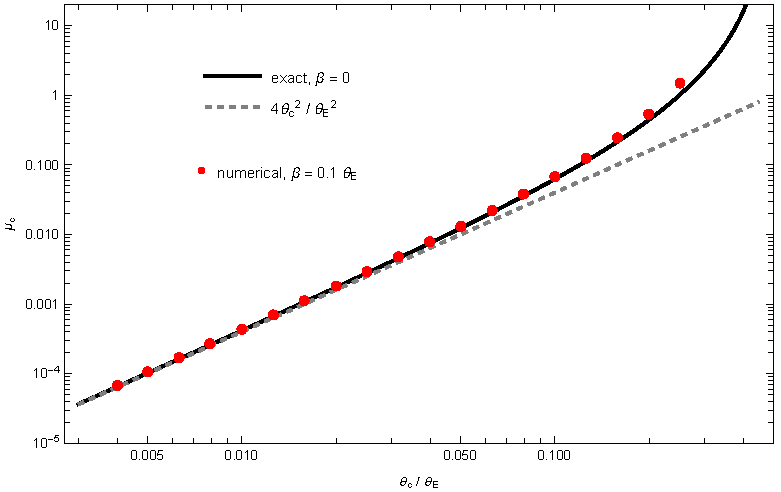
\includegraphics[width=0.7\textwidth]{../Figures/16_Odd_Images_Central/central_mag_vs_core.pdf}
    \caption{Magnification of the central image of an NIS as a function
    of core radius.  Solid: the on-axis closed form,
    eq.~\eqref{eq:oi_muc}; dashed: its small-core limit
    $4\theta_c^2/\thetaE^2$; points: numerical roots of the lens
    equation for $\ysrc=0.1\,\thetaE$, which lie within $6\%$ of the
    closed form for $\theta_c\le0.05\,\thetaE$.  The divergence as
    $\theta_c\to\thetaE/2$ is the radial critical circle shrinking onto
    the centre.  Generated by \texttt{odd\_images.wl}.}
    \label{fig:oi_muc}
\end{figure}

\begin{annotation}[Reading eq.~\eqref{eq:oi_muc}]
Three limits make the formula memorable.  (i) $\theta_c\to0$: the NIS
becomes the SIS, $\kappab_0\to\infty$ and $\mu_c\to0$ --- the central
image is pushed into the conical tip of Table~\ref{tab:oi_centres} with
zero flux.  (ii) $\theta_c\to\thetaE/2$: $\kappab_0\to1$, both
eigenvalues vanish at the centre, and the central image sits on a
degenerate (radial) critical point, so $\mu_c\to\infty$.  (iii) In
between, $\mu_c$ is small because $|\lambda|=\kappab_0-1$ is
\emph{large}: the summit of $\tau$ is sharply curved, and a sharply
curved stationary point is a strongly demagnified image.  Curvature
of $\tau$ is inverse brightness.
\end{annotation}

\paragraph{Why central images are rarely seen.}
Three effects conspire.  First, the demagnification of
eq.~\eqref{eq:oi_muc} for any realistically small core.  Second, the
central image sits on top of the lens galaxy's own bright nucleus, so
at optical wavelengths it is swamped; searches are done in the radio,
where the lens galaxy is usually faint.  Third, real galaxies are
cuspier than a cored isothermal sphere and host central black holes,
both of which suppress the image further (the next two sections).
\citet[][Sect.~6.2.2]{congdon_principles_2018} summarise model-based
expectations of typical central-image magnifications around $10^{-3}$,
with values as large as $0.1$ possible, and note that at the time of
writing a central image had been detected in only one galaxy-scale lens,
the radio quasar lens PMN~J1632$-$0033.  Conversely, a measured upper
limit on the central image's flux is a \emph{lower} limit on how cuspy
the centre is.

\begin{keybox}[The central image of a cored lens]
A supercritical core ($\kappab_0>1$) makes a third image, a maximum of
$\tau$ on the far side inside the radial critical curve, that
exists only for sources inside the radial caustic and has
\[
  \mu_c\simeq\frac{1}{(\kappab_0-1)^2}\simeq\frac{4\theta_c^2}{\thetaE^2}
  \quad(\theta_c\ll\thetaE).
\]
It is demagnified by the curvature of the summit of $\tau$.
\end{keybox}


% =====================================================================
\section{Steep Cusps Suppress the Central Image}
\label{sec:oi_steep}

A core is not the only way to keep the central image alive.  Consider
the power-law lens with $\thetaE$ as unit,
\begin{equation}
    \kappab(\theta) = \frac{3-\gp}{2}\,\theta^{1-\gp}, \qquad
    \alpha(\theta) = \operatorname{sgn}(\theta)\,|\theta|^{2-\gp},
    \qquad 1<\gp<2,
    \label{eq:oi_powerlaw}
\end{equation}
where $\gp$ is the slope of the three-dimensional density,
$\rho\propto r^{-\gp}$ ($\gp=2$ is isothermal; check G.1 verifies that
$\kappab$ and $\alpha$ are consistent).  The density diverges at the
centre, but, as noted in Section~\ref{sec:oi_hypotheses}, the
deflection is continuous, so there is a central image.

On the far side write $\theta=-x$ with $x>0$.  The lens equation reads
$\ysrc = x^{2-\gp}-x$, and for a small source offset the central root
has $x\ll1$, so $\ysrc\simeq x^{2-\gp}$, i.e.\ $x\simeq\ysrc^{1/(2-\gp)}$.
From eq.~\eqref{eq:oi_lambdas},
$\lambda_t = 1-x^{1-\gp}$ and $\lambda_r = 1-(2-\gp)\,x^{1-\gp}$; both
are large and negative for $x\to0$ (the image is a maximum), and
$\lambda_t\lambda_r\simeq(2-\gp)\,x^{2(1-\gp)}$ \annot{check G.2}.  Therefore
\begin{equation}
    \boxed{\;
    \mu_c \simeq \frac{1}{2-\gp}\;\left(\frac{\ysrc}{\thetaE}\right)^{2(\gp-1)/(2-\gp)}
    \;}
    \qquad (\ysrc\to0).
    \label{eq:oi_mu_powerlaw}
\end{equation}
The exponent $2(\gp-1)/(2-\gp)$ grows without bound as $\gp\to2$
\annot{check G.8}: steepening the cusp toward isothermal drives the central
image to zero flux for every source inside the radial caustic.  At
$\ysrc=0.1\,\thetaE$ the exact (numerical) values are $\mu_c=0.037$
for $\gp=1.5$, $3.1\times10^{-3}$ for $\gp=1.6$, $7.5\times10^{-5}$ for
$\gp=1.7$, and below $10^{-7}$ for $\gp=1.8$ \annot{checks G.4, G.6b, G.7}.  At
$\gp=1.2$ a source at $0.1\,\thetaE$ is already outside the radial
caustic and has no central image at all \annot{check G.6}.

\begin{annotation}[Leading order is a poor approximation at moderate offsets]
At $\gp=1.5$ and $\ysrc=0.1\,\thetaE$, eq.~\eqref{eq:oi_mu_powerlaw}
gives $\mu_c\simeq2\ysrc^2=0.02$, while the exact root gives $0.037$
--- almost a factor of two.  The corrections are of relative order
$x^{\gp-1}=\ysrc^{(\gp-1)/(2-\gp)}$, which for $\gp=1.5$ is
$\ysrc$ itself.  Use eq.~\eqref{eq:oi_mu_powerlaw} for its
\emph{scaling} with $\gp$; compute numbers from the exact root
(Exercise~\ref{ex:oi_powerlaw}).  At $\ysrc=10^{-4}\,\thetaE$ the two
agree to better than $1\%$ \annot{check G.5}.
\end{annotation}

The physical reading is the same as for the core: the steeper the cusp,
the more sharply peaked the summit of $-\psiL$, the more curved the
maximum of $\tau$, and the fainter the image.  A core and a shallow
cusp are two ways of rounding the summit; isothermal ($\gp=2$) is the
borderline at which the summit becomes a cone.


% =====================================================================
\section{A Central Point Mass Punctures the Surface}
\label{sec:oi_pointmass}

\subsection{The bare point mass: exactly two images}

For a point mass, $\alpha(\theta)=\thetaBH^2/\theta$ and
eq.~\eqref{eq:oi_lambdas} gives
\begin{equation}
    \lambda_r = 1 + \frac{\thetaBH^2}{\theta^2} > 0, \qquad
    \lambda_t = 1 - \frac{\thetaBH^2}{\theta^2}
    \label{eq:oi_pm_lambdas}
\end{equation}
\annot{checks E.1--E.2}.  Since $\lambda_r$ is positive \emph{everywhere}, no
point of the lens plane can host a maximum of $\tau$, and since
$\ysrc(\theta)$ is strictly increasing on each half-line, each side of
the lens has exactly one image.  These are the two roots
$\theta_\pm=\big(\ysrc\pm\sqrt{\ysrc^2+4\thetaBH^2}\big)/2$ of
Chapter~\ref{ch:lens_equation}, eq.~\eqref{eq:image_positions}: a
minimum at $\theta_+>\thetaBH$ and a saddle at $\theta_-<0$ inside the
Einstein ring, with $n_+-n_-=0$, exactly as eq.~\eqref{eq:oi_index_pm}
demands for $g=1$ \annot{checks E.3--E.4}.

\subsection{A point mass inside a cored lens}

Now put a point mass at the centre of an NIS --- a supermassive black
hole at the centre of a galaxy.  The one-dimensional map becomes
\begin{equation}
    \ysrc(\theta) = \theta - \thetaE\,\frac{\sqrt{\theta^2+\theta_c^2}-\theta_c}{\theta}
                   - \frac{\thetaBH^2}{\theta}.
    \label{eq:oi_nisbh_map}
\end{equation}
Multiplying by $\theta$ and squaring as before gives a quartic \annot{check B.4}, so there are at most four images, and by eq.~\eqref{eq:oi_index_pm}
with $g=1$ their number is even.  The radial eigenvalue is the key
object.  Using $\theta^2=s^2-\theta_c^2$ it factorises neatly:
\begin{equation}
    \theta^2\lambda_r = h(s) + \thetaBH^2, \qquad
    h(s) \equiv (s-\theta_c)\left(s+\theta_c-\frac{\thetaE\theta_c}{s}\right),
    \qquad s=\sqrt{\theta^2+\theta_c^2}
    \label{eq:oi_theta2lr}
\end{equation}
\annot{check H.1}.

\begin{derivation}[Factorising $\theta^2\lambda_r$]
Differentiate the NIS deflection of eq.~\eqref{eq:oi_nis}, using
$\dd s/\dd\theta=\theta/s$:
\[
  \deriv{\alpha}{\theta}
  = \thetaE\left[\frac{1}{s} - \frac{s-\theta_c}{\theta^2}\right].
\]
Add the point-mass term $\dd(\thetaBH^2/\theta)/\dd\theta=-\thetaBH^2/\theta^2$
and multiply by $\theta^2$:
\[
  \theta^2\lambda_r = \theta^2 - \frac{\thetaE\theta^2}{s}
                    + \thetaE(s-\theta_c) + \thetaBH^2 .
\]
Replace $\theta^2$ by $s^2-\theta_c^2=(s-\theta_c)(s+\theta_c)$ in the
first two terms and pull out the common factor $(s-\theta_c)$:
\[
  (s-\theta_c)\left[(s+\theta_c) - \frac{\thetaE(s+\theta_c)}{s} + \thetaE\right]
  = (s-\theta_c)\left[s+\theta_c-\frac{\thetaE\theta_c}{s}\right].
\]
For $\thetaBH=0$ the radial critical curve is $h(s)=0$ with
$s>\theta_c$, i.e.\ $s^2+\theta_c s-\thetaE\theta_c=0$, which is
eq.~\eqref{eq:oi_nis_radial}.  With $\thetaBH\neq0$, $h(s)+\thetaBH^2=0$
is the cubic $s^3-(\theta_c^2+\thetaE\theta_c-\thetaBH^2)\,s+\thetaE\theta_c^2=0$
\annot{check H.18}.
\end{derivation}

\paragraph{Two radial critical circles.}
The function $h(s)$ vanishes at $s=\theta_c$ (the centre), dips to a
negative minimum, and rises again.  Adding $\thetaBH^2>0$ lifts the
whole curve.  For a small black hole $h+\thetaBH^2$ still dips below
zero, so it has two zeros: an inner critical circle $r_1$ created by
the black hole and the (slightly displaced) radial critical circle
$r_2$ of the NIS.  On the far side, the map $\ysrc(\theta)$ therefore
rises from $-\infty$, reaches a local maximum $\ysrc_{\rm out}$ at
$\theta=-r_2$ (the radial caustic), falls to a local minimum
$\ysrc_{\rm in}$ at $\theta=-r_1$ (a new, inner caustic), and then
rises to $+\infty$ as $\theta\to0^-$.  On the near side there is a
single image, the minimum.  Counting crossings of a source value
$\ysrc$:
\begin{center}
\small
\begin{tabular}{lcl}
\toprule
Source & $N$ & Images \\
\midrule
$\ysrc<\ysrc_{\rm in}$ & 2 & minimum; far-side saddle outside $r_2$ \\
$\ysrc_{\rm in}<\ysrc<\ysrc_{\rm out}$ & 4 & minimum; saddle; \textbf{central maximum}; saddle next to the black hole \\
$\ysrc>\ysrc_{\rm out}$ & 2 & minimum; saddle next to the black hole \\
\bottomrule
\end{tabular}
\end{center}
The census is verified on source grids in checks H.10--H.13, with
$n_+-n_-=0$ throughout.  The central maximum survives only in the
middle band, and next to it the black hole has created a \emph{second}
faint image --- a saddle hugging the puncture, visible in the middle
column of Figure~\ref{fig:oi_arrival}.  This matches the picture of
\citet{mao_witt_koopmans_2001} as summarised in Sect.~6.2.2 of
\citet{congdon_principles_2018}: above a threshold black-hole mass an
NIS cannot form a central image at all; below it the central image may
become unobservably faint, or a second central image may form.

\paragraph{A small black hole already matters.}
For $\thetaBH\to0$ the inner critical circle sits where
$(\kappab_0-1)\theta^2\simeq\thetaBH^2$, and the inner caustic has
radius
\begin{equation}
    \ysrc_{\rm in} \simeq 2\,\thetaBH\sqrt{\kappab_0-1}
    \label{eq:oi_yin}
\end{equation}
\annot{check H.14}.  It grows \emph{linearly} in $\thetaBH$, i.e.\ as the square
root of the black-hole mass, so even a small black hole removes the
central image for every source closer to the axis than $\ysrc_{\rm in}$
\annot{check H.15}.  For $\theta_c=0.1\,\thetaE$ ($\kappab_0=5$), a point mass
with $\thetaBH=0.082\,\thetaE$ already removes it for every source within
$0.3\,\thetaE$ of the axis \annot{check H.16}.

\begin{derivation}[The inner caustic for a small black hole]
Near the centre $\alpha_{\rm NIS}\simeq\kappab_0\theta$, so on the far
side ($\theta=-x$, $x>0$)
\[
  \ysrc(-x) \simeq (\kappab_0-1)\,x + \frac{\thetaBH^2}{x}.
\]
This is a sum of a rising and a falling term; its minimum is at
$x_1=\thetaBH/\sqrt{\kappab_0-1}$ (the inner critical circle $r_1$),
where $\ysrc = 2\thetaBH\sqrt{\kappab_0-1}$.  The approximation needs
$x_1\ll\theta_c$, i.e.\ $\thetaBH\ll\theta_c\sqrt{\kappab_0-1}$.
\end{derivation}

\subsection{The critical black-hole mass}

As $\thetaBH$ grows, the dip of $h(s)+\thetaBH^2$ becomes shallower, the
two critical circles approach each other, and at a critical mass they
merge and disappear.  Beyond it $\lambda_r>0$ everywhere, $\ysrc(\theta)$
is monotonic on each side, and every source has exactly two images,
a minimum and a saddle, with no maximum anywhere.  The boundary is
$\thetaBH^2=-\min_s h(s)$.  Setting $h'(s)=2s-\thetaE\theta_c^2/s^2=0$
gives $s_\star^3=\thetaE\theta_c^2/2$ (which lies at $\theta>0$ exactly
when the core is supercritical, $\theta_c<\thetaE/2$; checks H.2--H.3),
and $h(s_\star)=3s_\star^2-\theta_c^2-\thetaE\theta_c$, so
\begin{equation}
    \boxed{\;
    \theta_{\bullet,\rm crit}^2
    = \theta_c(\thetaE+\theta_c) - 3\left(\frac{\thetaE\theta_c^2}{2}\right)^{2/3}
    \;}
    \label{eq:oi_ucrit}
\end{equation}
\annot{checks H.4--H.6}.  It vanishes as $\theta_c\to\thetaE/2$, where the NIS
radial critical curve itself shrinks to the centre, and tends to
$\thetaE\theta_c$ as $\theta_c/\thetaE\to0$.
For $\theta_c=0.1\,\thetaE$ it gives $\theta_{\bullet,\rm crit}^2=0.0223\,\thetaE^2$
($\theta_{\bullet,\rm crit}=0.149\,\thetaE$), and for $\theta_c=0.2\,\thetaE$,
$0.0190\,\thetaE^2$ ($0.138\,\thetaE$) \annot{check H.7}.  The closed form agrees
with a direct numerical minimisation of $\theta^2\lambda_r$, and the
minimum of $\lambda_r$ changes sign across it \annot{checks H.8--H.9, H.11--H.12}.

\begin{derivation}[Evaluating $h$ at its minimum]
Write $h(s)=s^2-\theta_c^2-\thetaE\theta_c+\thetaE\theta_c^2/s$ (expand
eq.~\eqref{eq:oi_theta2lr}).  At $s_\star$, $\thetaE\theta_c^2=2s_\star^3$, so
the last term is $2s_\star^2$ and $h(s_\star)=3s_\star^2-\theta_c^2-\thetaE\theta_c$.
Then $\theta_{\bullet,\rm crit}^2=-h(s_\star)=\theta_c^2+\thetaE\theta_c-3s_\star^2$
with $s_\star^2=(\thetaE\theta_c^2/2)^{2/3}$.  Because $h(s)+\thetaBH^2$
is $\theta^2\lambda_r$, the condition ``its minimum touches zero'' is
the simultaneous solution of $\lambda_r=0$ and $\dd\lambda_r/\dd\theta=0$,
i.e.\ $\dd\ysrc/\dd\theta=\dd^2\ysrc/\dd\theta^2=0$: the two critical
circles coincide.
\end{derivation}

\begin{figure}[ht]
    \centering
    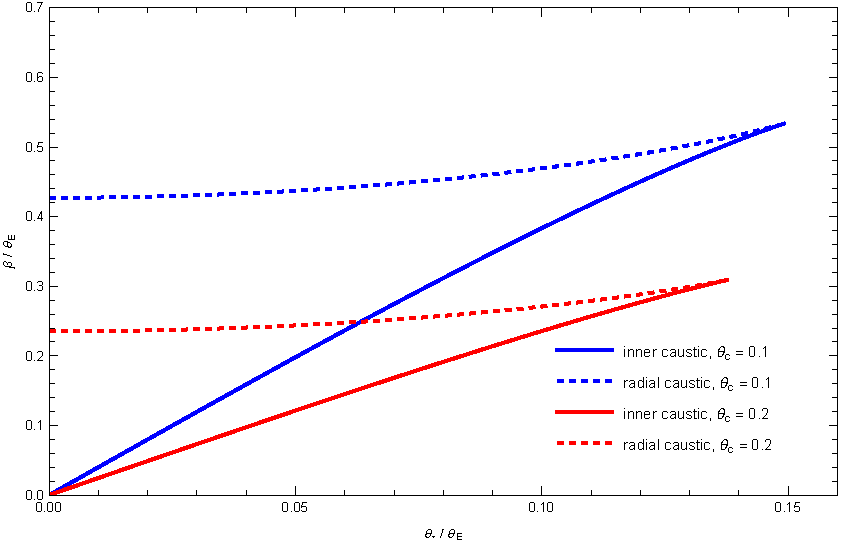
\includegraphics[width=0.72\textwidth]{../Figures/16_Odd_Images_Central/central_image_phase.pdf}
    \caption{Where a central image can exist, for an NIS with a central
    point mass.  For each black-hole Einstein radius $\thetaBH$ the
    central image exists only for sources between the inner caustic
    (solid; eq.~\ref{eq:oi_yin} at small $\thetaBH$) and the radial
    caustic (dashed).  The two curves meet and end at
    $\theta_{\bullet,\rm crit}$, eq.~\eqref{eq:oi_ucrit}; above it no
    source has a central image.  Blue: $\theta_c=0.1\,\thetaE$; red:
    $\theta_c=0.2\,\thetaE$.  Generated by \texttt{odd\_images.wl}.}
    \label{fig:oi_phase}
\end{figure}

\begin{keybox}[The annihilation boundary]
A central point mass of Einstein radius $\thetaBH$ in a cored lens
creates an inner critical circle around itself.  As $\thetaBH$ grows,
this circle and the lens's own radial critical circle approach, and at
$\thetaBH=\theta_{\bullet,\rm crit}$ (eq.~\ref{eq:oi_ucrit} for the NIS)
they merge and annihilate.  Below the boundary a source can have four
images (minimum, saddle, central maximum, black-hole saddle) or two;
above it every source has exactly two (minimum and saddle), and the
radial caustic --- with every image associated with it --- no longer
exists.  For any fixed source, the central maximum disappears earlier,
by merging with the black-hole saddle when the inner caustic sweeps
past the source.
\end{keybox}

\begin{bridge}[Forward to Chapter~\ref{ch:central_mass_bias}]
Chapter~\ref{ch:central_mass_bias} studies the same competition with a
power-law deflector instead of a cored one.  The algebra changes, but
the logic of eq.~\eqref{eq:oi_ucrit} carries over unchanged: the
boundary is the simultaneous solution of $\dd\ysrc/\dd\theta=0$ and
$\dd^2\ysrc/\dd\theta^2=0$, and above it the radial critical curve is
gone.  That chapter calls this the annihilation boundary and uses it to
bound how massive a central black hole can be in a lens that still
shows a radial image.  The power-law-plus-point-mass lens itself is the
subject of Chapter~\ref{ch:power_law_point_mass}.
\end{bridge}

\begin{annotation}[Two different mergers --- do not confuse them]
For a \emph{fixed source}, increasing $\thetaBH$ first makes the inner
caustic sweep outward past the source; at that moment the central
maximum merges with the black-hole saddle (a $+1$ and a $-1$ image
annihilate, so $n_+-n_-$ is unchanged) and the count drops from four to
two.  For the \emph{lens as a whole}, at $\theta_{\bullet,\rm crit}$ the
inner and radial caustics merge, so no source anywhere can have four
images.  The first is a source crossing a fold caustic; the second is
the disappearance of the caustic pair itself.  In
Figure~\ref{fig:oi_phase}, a horizontal line at fixed $\ysrc$ crosses
the solid curve (first merger) before the curves end (second).
\end{annotation}


% =====================================================================
\section{A Degeneracy: Inner Slope versus Central Mass}
\label{sec:oi_degeneracy}

Sections~\ref{sec:oi_central}--\ref{sec:oi_pointmass} identified three
knobs that control the central image:
\begin{itemize}[nosep]
    \item a \textbf{core} rounds the summit of $\tau$ and makes a central
          image with $\mu_c\propto\theta_c^2$;
    \item a \textbf{steep cusp} sharpens the summit and suppresses the
          image as $\gp\to2$, eq.~\eqref{eq:oi_mu_powerlaw};
    \item a \textbf{central point mass} punctures the summit, creates an
          inner caustic of radius $\propto\thetaBH$, and above a critical
          mass removes the central image altogether.
\end{itemize}
The last two act in the same direction.  A faint or absent central
image can be produced by a steep inner profile, by a black hole in a
shallower profile, or by a combination; the central-image flux alone
does not separate them.
\citet[][Sect.~6.2.2]{congdon_principles_2018} make the same point:
central images are demagnified by black holes, so a given central-image
magnification is to some extent degenerate between black-hole mass and
inner density profile.

The degeneracy also reaches the images we \emph{do} see.  The radial
critical curve, whose existence is decided by the same inner mass
distribution, controls whether a radial arc or a radial image of an
extended source can form.  Chapter~\ref{ch:central_mass_bias}
quantifies how a black hole that is left out of the model biases the
inferred lens parameters, and Chapter~\ref{ch:msd_kinematics} turns to
the mass-sheet degeneracy and to stellar kinematics, the independent
handle on the mass profile that is needed when lensing alone cannot fix
it.

\begin{annotation}[Why the centre is a separate measurement]
Lensing constrains the mass \emph{inside} the Einstein radius very well
and its radial distribution there poorly.  The central image is one of
the few probes of the innermost $\sim0.1\,\thetaE$, and
Sections~\ref{sec:oi_central}--\ref{sec:oi_pointmass} show that it
responds to a core, a cusp and a black hole in ways that partly cancel.
Treat a central-image non-detection as a constraint on a
\emph{combination} of inner slope and central mass, not on either alone.
\end{annotation}


% =====================================================================
\section{Summary}
\label{sec:oi_summary}

\begin{itemize}
    \item Images are the zeros of $\nabla\tau$; each carries index
          $\operatorname{sgn}\mu=\pm1$.  A maximum of $\tau$ requires
          $\kappab>1+|\gammaL|$, so it can only sit near the centre of
          the lens.

    \item If the deflection is continuous and bounded, the indices sum
          to the winding at infinity: $n_+-n_-=1$ and $N=1+2n_-$
          (Burke).  What matters is continuity of $\vecalpha$: a
          power-law cusp with $1<\gp<2$ has infinite central density
          yet still obeys the theorem.

    \item A point mass violates continuity and boundedness of
          $\vecalpha$ at one point.  The puncture carries index $+1$, so
          $n_+-n_-+g=1$: one point mass makes the image count even.  A
          bare point mass has $\lambda_r=1+\thetaBH^2/\theta^2>0$
          everywhere and exactly two images.

    \item The central image of an NIS is a maximum on the far side
          inside the radial critical curve, arrives last, and has
          $\mu_c=(1-\kappab_0)^{-2}\simeq4\theta_c^2/\thetaE^2$.  Small
          cores make it many magnitudes fainter than the source, and it
          sits on the bright galaxy nucleus.

    \item Steepening a power-law cusp suppresses the central image as
          $\mu_c\propto(\ysrc/\thetaE)^{2(\gp-1)/(2-\gp)}$, which vanishes
          as $\gp\to2$.

    \item A central point mass in a cored lens creates an inner caustic
          of radius $\simeq2\thetaBH\sqrt{\kappab_0-1}$ inside which the
          central image is destroyed, and above
          $\theta_{\bullet,\rm crit}^2=\theta_c(\thetaE+\theta_c)-3(\thetaE\theta_c^2/2)^{2/3}$
          it removes the radial critical curve and every central image.
          This is the annihilation boundary of
          Chapter~\ref{ch:central_mass_bias}.

    \item A steep cusp and a central black hole both suppress the
          central image: its flux constrains a combination of the two.
\end{itemize}


% =====================================================================
\section{Problems}
\label{sec:oi_problems}

\begin{exercise}[Fermat gradient and Hessian]
\label{ex:oi_gradient_hessian}
For an arbitrary smooth potential $\psiL(\theta_1,\theta_2)$:
\begin{enumerate}[label=(\alph*)]
    \item Show that $\nabla_{\vectheta}\tau=0$ is the lens equation.
    \item Show that $\nabla\nabla\tau=\Amat$, and that
          $\operatorname{tr}\Amat=2(1-\kappab)$.
    \item Using eq.~\eqref{eq:oi_eigen}, show that the image type is
          fixed by the signs of $\det\Amat$ and $\operatorname{tr}\Amat$.
\end{enumerate}
\end{exercise}

\begin{exercise}[Five images of a cored elliptical lens]
\label{ex:oi_five_images}
Use eq.~\eqref{eq:oi_index_sum} to show that a source inside both the
tangential and the radial caustic of a smooth cored elliptical lens,
which sees four bright images, must have a fifth, and identify the type
and parity of each.  Then verify your answer numerically with the
softened elliptical potential
$\psiL=\sqrt{s^2+(1-e)\theta_1^2+(1+e)\theta_2^2}$, $s=0.25$, $e=0.3$,
and source $\vecbeta=(0.05,0.03)$.
\end{exercise}

\begin{exercise}[The NIS central image]
\label{ex:oi_nis_central}
For the NIS, eq.~\eqref{eq:oi_nis}:
\begin{enumerate}[label=(\alph*)]
    \item Show that $\lambda_t(0)=\lambda_r(0)=1-\kappab_0$, and hence
          that the centre is a maximum of $\tau$ if and only if
          $0<\theta_c<\thetaE/2$.
    \item Derive eq.~\eqref{eq:oi_muc} and its small-core limit.
    \item For a small source offset, show that the central image lies at
          $\theta\simeq-\ysrc/(\kappab_0-1)$.  Evaluate for
          $\theta_c=0.1\,\thetaE$, $\ysrc=0.01\,\thetaE$.
    \item Show that as $\theta_c\to0$ the deflection tends to the SIS
          value and the central image's magnification tends to zero.
\end{enumerate}
\end{exercise}

\begin{exercise}[Point masses change the parity of the count]
\label{ex:oi_puncture}
\begin{enumerate}[label=(\alph*)]
    \item Show that the winding number of $\nabla\tau$ around a small
          circle centred on a point mass is $+1$, whatever the source
          position.
    \item Deduce eq.~\eqref{eq:oi_index_pm} for $g$ point masses
          embedded in a smooth lens, and show that each added point mass
          changes the parity of the image count, while $N+g$ stays odd.
    \item Check this against the NIS-plus-point-mass census of
          Section~\ref{sec:oi_pointmass}: compare the image counts with
          and without the black hole for the same source.
\end{enumerate}
\end{exercise}

\begin{exercise}[The tip of the SIS]
\label{ex:oi_sis_tip}
For the SIS, $\nabla\tau=\vectheta-\vecbeta-\thetaE\hat{\vectheta}$.
\begin{enumerate}[label=(\alph*)]
    \item Show that on a circle of radius $\epsilon\to0$ around the
          origin the field winds once if $|\vecbeta|<\thetaE$ and not at
          all if $|\vecbeta|>\thetaE$.
    \item Combine with the SIS image parities to show that the sum of
          the image indices and the tip index equals $1$ in both cases.
          Which circle in the source plane plays the role of a caustic?
\end{enumerate}
\end{exercise}

\begin{exercise}[The critical black-hole mass]
\label{ex:oi_critical_mass}
\begin{enumerate}[label=(\alph*)]
    \item Show that eq.~\eqref{eq:oi_ucrit} can be written exactly as
          $\theta_{\bullet,\rm crit}^2=\thetaE\theta_c-3\cdot2^{-2/3}\thetaE^{2/3}\theta_c^{4/3}+\theta_c^2$,
          and that $\theta_{\bullet,\rm crit}^2/(\thetaE\theta_c)\to1$
          as $\theta_c/\thetaE\to0$.
    \item Evaluate $\theta_{\bullet,\rm crit}$ for $\theta_c=0.05\,\thetaE$.
    \item The black hole's mass relative to the NIS mass inside $\thetaE$
          is $\mBH=\thetaBH^2/[\thetaE\,\alpha(\thetaE)]$.  Evaluate the
          critical $\mBH$ for $\theta_c=0.1\,\thetaE$.
\end{enumerate}
\end{exercise}

\begin{exercise}[A shallow cusp]
\label{ex:oi_powerlaw}
For the power-law lens, eq.~\eqref{eq:oi_powerlaw}, with $\gp=1.5$:
\begin{enumerate}[label=(\alph*)]
    \item Solve the far-side lens equation exactly (substitute
          $x=w^2$) and show that a source at $\ysrc<\thetaE/4$ has three
          images.
    \item Compute the exact central-image magnification at
          $\ysrc=0.1\,\thetaE$ and compare with eq.~\eqref{eq:oi_mu_powerlaw}.
    \item Repeat (b) numerically for $\gp=1.8$ and comment.
\end{enumerate}
\end{exercise}
